%
% File acl2019.tex
%
%% Based on the style files for ACL 2018, NAACL 2018/19, which were
%% Based on the style files for ACL-2015, with some improvements
%%  taken from the NAACL-2016 style
%% Based on the style files for ACL-2014, which were, in turn,
%% based on ACL-2013, ACL-2012, ACL-2011, ACL-2010, ACL-IJCNLP-2009,
%% EACL-2009, IJCNLP-2008...
%% Based on the style files for EACL 2006 by 
%%e.agirre@ehu.es or Sergi.Balari@uab.es
%% and that of ACL 08 by Joakim Nivre and Noah Smith

\documentclass[11pt,a4paper]{article}
\usepackage[hyperref]{acl2019}
\usepackage{times}
\usepackage{latexsym}
\usepackage{url}
\usepackage{color}
\usepackage{enumerate}
\usepackage{balance}
\usepackage{graphics}
\usepackage{graphicx}
\usepackage{multirow}
\usepackage{caption} 
\usepackage{makecell}
\usepackage{xcolor}
\usepackage{url}

\usepackage{epsfig}
\usepackage{amssymb}
\usepackage{amsmath}
\usepackage{amsfonts}

\captionsetup[table]{skip=6pt}

\aclfinalcopy % Uncomment this line for the final submission
%\def\aclpaperid{***} %  Enter the acl Paper ID here

%\setlength\titlebox{5cm}
% You can expand the titlebox if you need extra space
% to show all the authors. Please do not make the titlebox
% smaller than 5cm (the original size); we will check this
% in the camera-ready version and ask you to change it back.

\newcommand\BibTeX{B\textsc{ib}\TeX}

\title{
  Mood Classification Using Song Lyrics\\
  Introduction to Natural Language Processing - Project
}

\author{Abhiram Ravi Bharadwaj \\
  Rochester Institute of Technology \\
  Department of Computer Science \\
  \texttt{ab8136@rit.edu} \\}

\date{}

\begin{document}
\maketitle
\begin{abstract}
  With the recent advancements in music streaming services like Spotify, YouTube Music, Amazon Prime Music etc, it has become a major avenue to suggest music to the audience. Suggesting valid music to the audience requires understanding the mood of the audience and recommending songs based on the mood. An obvious necessity is to be able to classify music into the various different moods so as to be able to recommend music. This project aims at successfully classifying musing into one of various different moods.\\

\end{abstract}

\section{Introduction}
\label{introduction}
The current technology allows for people to be connected to the internet at all times. This means that there is very little need for any media to be stored locally on any device. That media includes music as well. With the recent advancements in music streaming services like Spotify, YouTube Music, Amazon Prime Music etc, it has become a major avenue to suggest music to the audience. Suggesting valid music to the audience requires understanding the mood of the audience and recommending songs based on the mood. An obvious necessity is to be able to classify music into the various different moods so as to be able to recommend music.\\
This project aims at successfully classifying musing into one of various different moods. This task can be accomplished in two ways, either by considering the audio of the songs or by looking at the lyrics in the songs. This project looks at the latter approach by classifying lyrics into various moods. There are some particular steps that would need to be followed to accomplish this:
\begin{itemize}
  \item \textbf{Data collection} is the first step in any machine learning process. Same is the case in this project. A corpus of song lyrics was needed. A corpus of nearly 2,000 song lyrics from four genres:
  \begin{enumerate}
    \item Rock
    \item Country
    \item Rap/Hip Hop
    \item Reggae
  \end{enumerate}
  was obtained.
  \item \textbf{Data annotation} is the process of labelling data into the various classes of interest. In this project the data was annotated using the GEMS scale for music emotion. At least one category was assinged to each instance of the data. The categories and definitions are mentioned in Table \ref{categories}.
  \begin{table}[!htbp]
  \centering
  \caption{List of categories with the definition of the categories according to GEMS.}
  \label{categories}
  \scalebox{0.9}{
    \begin{tabular}{|c|c|} \hline
    \textbf{Category} & \textbf{Definition}\\ \hline
    Amazement & Feeling of wonder and happiness.\\ \hline
    Solemnity & Feeling of transcendence.\\ \hline
    Tenderness & Sensuality, affection, feeling of love.\\ \hline
    Nostalgia & \makecell{Dreamy, melancholy,\\sentimental feelings.}\\ \hline
    Calmness & Relaxation, serenity, meditativeness.\\ \hline
    Power & \makecell{Feeling strong, heroic, triumphant,\\energetic.}\\ \hline
    Joyful Activation & \makecell{Feels like dancing, bouncy feeling,\\animated, amused.}\\ \hline
    Tension & Nervous, impatient, irritated.\\ \hline
    Sadness & Depressed, sorrowful.\\ \hline
    \end{tabular}
  }
  \end{table}
  \item \textbf{Data cleaning} is essentially preprocessing data. Once the data has been annotated, it is prone to having a lot of junk values as well. The quality of work of annotators cannot ever be guaranteed since annotation is subjective. So instead of annotating the data again, it would just be easier and save a lot of resources to just clean the data. This is the step where junk data would also be removed.\\
  Most song lyrics are usually obtained by speech to text machines \cite{gupta2019automatic, anna2016retrieval, annamaria2010recognition} and this usually leads to retrieval of some unwanted data as well. This could be due to the singer humming a tune or instruments sounding like people etc.
  \item \textbf{Classification} is the logical next step once the data has been cleaned and ready to be consumed by the machine learing models. Classification involves training a model into being able to classify the song lyrics into one of the classes provided. Typically multiple classification algorithms like k-nearest neighbour \cite{guo2004knn}, support vector networks \cite{Cortes:1995:SN:218919.218929}. In this project we look at at least two different classification algorithms and compare their results. This process is discussed in more detail in section \ref{methods}.
  \item \textbf{Analysis}. Once the classification model is built, it needs to be tested to check how well it performs. This could be done by looking at various scores and also visualisations. In this project, visualisations are not considered.
\end{itemize}
Section \ref{relatedwork} briefly talks about some related work to this project. In section \ref{data} the data used in this project is explained with some of the pre-processing done on it. The crux of the work done is explained in section \ref{methods}. Section \ref{results} explains the results obtained from the experiments and section \ref{conclusion} concludes this project's outcomes.

\section{Related Work}
\label{relatedwork}
Describe related work on lyrics/music classification. 1pg
Attributing to the increased importance of recommender systems, a lot of recent research work has focussed on building better recommendation systems. Music also has grown into needing a recommendation system due to the vast popularity of streaming services. This need draws a lot of attention and some good research has been done. One such work is by Giammusso et al. \cite{giammussopredicting} who propose an approach to classifying songs into four different classes:
\begin{itemize}
  \item relaxed
  \item happy
  \item sad
  \item angry
\end{itemize}
In their work, they look at identifying stylometric, structural, orientation and vocabulary based features which they extract from lyrics. These featues include attributes like the proportion of verbs in various tenses and also some POS tags.\\
Recommendation systems also rely on identifying what songs are popular or rather in predicting what songs might get popular and suggesting those songs to its subscribers. This area was tapped on by Barman et al. \cite{barman2019decoding}. Of the various different approaches to identifying popular songs, they use lyrics. They note that the style of lyrics have a very obvious difference between popular songs and other songs. Another aspect that they consider is the bias in songs. This, according to them is similar to the bias that humans show. This tells that song lyrics reflect the biases in society. Truly the work of Giammusso et al.\cite{giammussopredicting} and Barman et al. \cite{barman2019decoding} can be thought of as previous work rather than related work.\\
The research that is closest to what this project aims at doing was done by Hu et al. \cite{hu2009lyric}. They showcase how important it is in evaluating music information retrieval systems that can access the mood dimension of music in an automated manner. Their work looks deeply into twenty two systems that have been evaluated and looks to address the important issues that were raised during those evaluations. They note that due to the subjectivity of music perception, arriving at a ground truth for the mood of a song can be difficult. This is one of the issues that was encountered during the course of this project as well. Asking people to annotate data is easy but there is no strong distinction between what is right and what is wrong. This project can be construed as a miniature of the work done by Hu et al. \cite{hu2009lyric}. Although Hu et al. \cite{hu2009lyric} used an SVM with a linear kernel and default parameters, this project will test other models and fine tune the parameters aiming to improve the accuracy of classification.\\
A problem that is similar to mood classification is genre detection. Song prediction can be done hierarchically as to first predict the mood and then predict the song. Selecting the song could be done by choosing a genre so it can be seen that genre and mood are corelated. Fell et al. \cite{fell2014lyrics} build a lyrics based classification model that performs genre detection, distingushing best and worst songs and determining the approximate publication time of a song. Looking at all these research, it is evident that performing bag of words as described in section \ref{bow} is an important task.

\section{Data}
\label{data}
As mention in section \ref{introduction}, the data consisted of around 2,000 instances. Once the data was collected, a group of 24 students from Rochester Institute of Technology were assigned the task of annotating the data. Each one of the 24 were requested to annotate a minimum of 200 instances. A particular instance was annotated by three different students to ensure the best possible annotation. Students were instructed to assign every record at least one class among the given nine class labels.\\ 
Once the annotation was done, every record had more than one class label associated with it. As part of the data pre-processing, the data was converted into two forms:
\begin{enumerate}
  \item The first type was the \textbf{single label}. In this dataset, all the records were assigned just one class. The class assigned was decided by a max-pooling from all the annotations by the students. A sample of this data is shown in Figure \ref{single_label}.
  \begin{figure}[!htbp]
  \begin{center}
  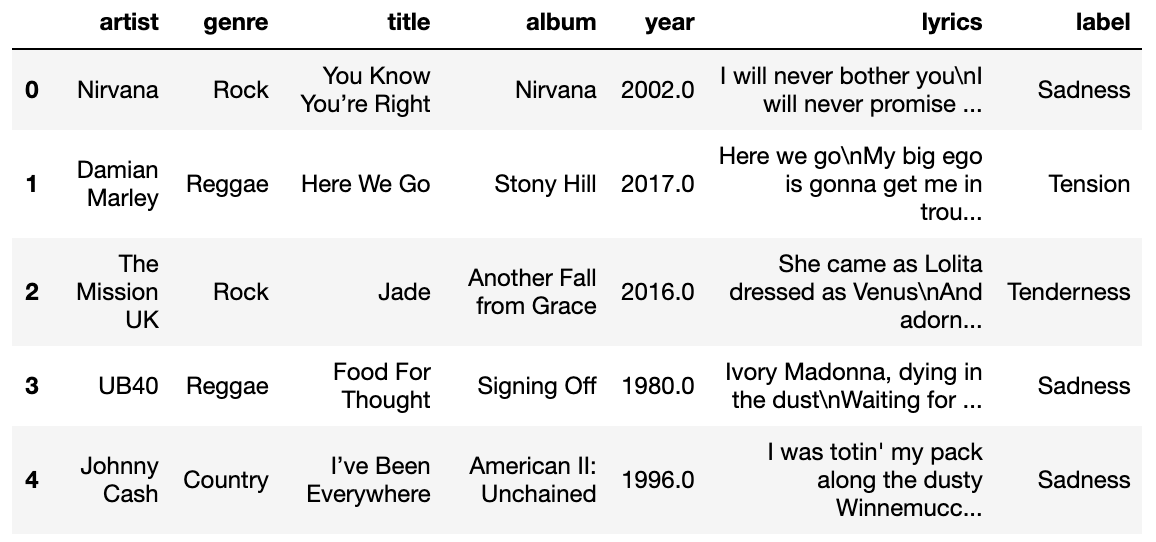
\includegraphics[width=3in]{1_single_label.png}
  \caption{Sample of the single labelled data.}
  \label{single_label}
  \end{center}
  \end{figure}

  \item The second type was the \textbf{multi label}. In this dataset, all of the unique class labels that the students had assigned were present. A sample of this data is shown in Figure \ref{multi_label}.
  \begin{figure}[!htbp]
  \begin{center}
  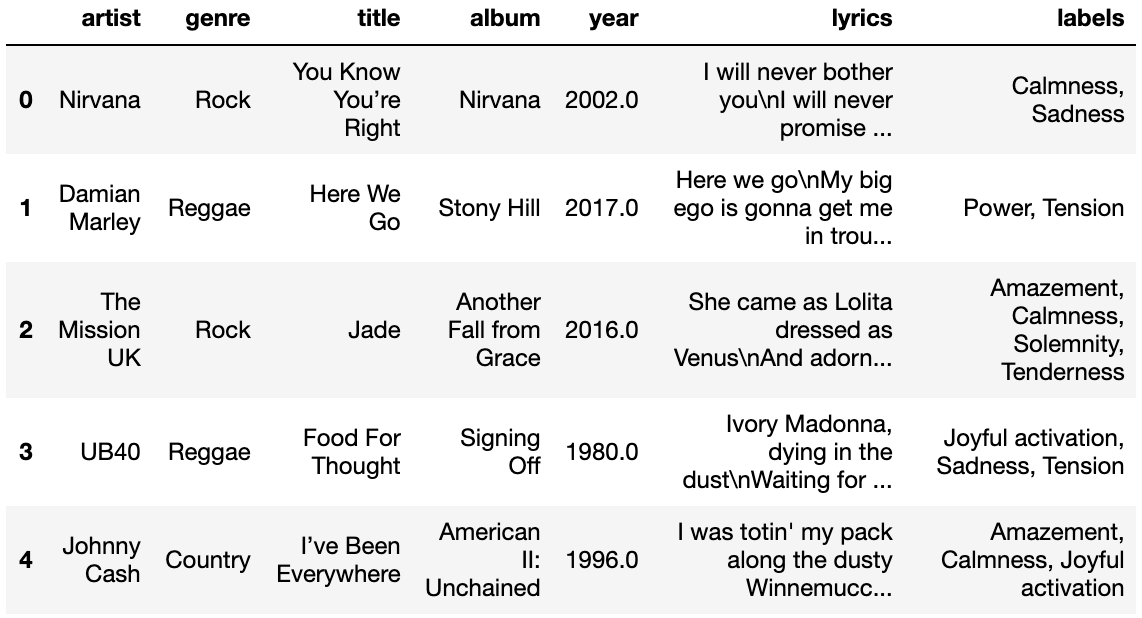
\includegraphics[width=3in]{2_multi_label.png}
  \caption{Sample of the multi labelled data.}
  \label{multi_label}
  \end{center}
  \end{figure}

\end{enumerate}

For the purpose of this project, only the single labelled data is used. Specifically, the data for three classes is extracted and a model is built to classify songs into one of these three classes. The classes selected are:
\begin{itemize}
  \item Sadness
  \item Tenderness
  \item Tension
\end{itemize}
Table \ref{distribution} shows the distribution of data into these three classes. These three classes had the most number of instances in them and hence these were chosen.
\begin{table}[!htbp]
  \centering
  \caption{Distribution into the three classes in single labelled data.}
  \label{distribution}
  \begin{tabular}{|c|c|} \hline
  \textbf{Category} & \textbf{Count}\\ \hline
  Sadness & 569\\ \hline
  Tenderness & 326\\ \hline
  Tension & 265\\ \hline
  \end{tabular}
\end{table}

\begin{figure}[!htbp]
  \begin{center}
  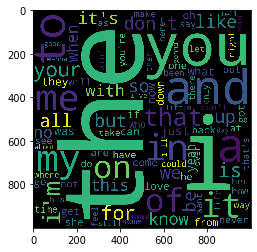
\includegraphics[width=3in]{3_sadness.png}
  \caption{Word cloud obtained by plotting the words labelled as sadness.}
  \label{sadness}
  \end{center}
\end{figure}

Classification of songs is not a trivial task. It cannot be simply achieved by computing the frequency of words belonging to each label and looking at patterns in them. Building such complex models is a necessity. Figures \ref{sadness}, \ref{tenderness} and \ref{tension} show the word clouds obtained by visualising the top 200 words belonging to each class label.

\begin{figure}[htb]
  \begin{center}
  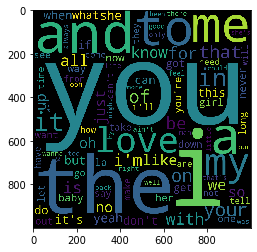
\includegraphics[width=3in]{4_tenderness.png}
  \caption{Word cloud obtained by plotting the words labelled as tenderness.}
  \label{tenderness}
  \end{center}
\end{figure}

\begin{figure}[htb]
  \begin{center}
  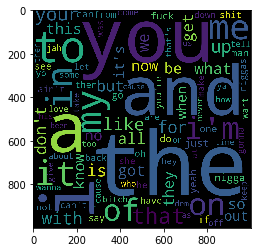
\includegraphics[width=3in]{5_tension.png}
  \caption{Word cloud obtained by plotting the words labelled as tension.}
  \label{tension}
  \end{center}
\end{figure}

Before visualising these word clouds, the data had to be cleaned. Without cleaning the data consisted of a lot of punctuations and symbols. This cleaning was done using packages provided by nltk \cite{nltk}. To clean the data, it first had to be prepared in a way that it could be consumed by the tokenizer and to achieve that the data was first segmented. Once the data was cleaned, data points corresponding to each one of the three classes were filtered out and passed to the word cloud visualiser. The visualisation was done using matplotlib \cite{matplotlib}.

\section{Methods}
\label{methods}
After the data has been curated, it is now ready to be consumed by machine learning models.

\subsection{Technology Used}
\label{techstack}
A bunch of technologies and libraries were used in building this song classifier. Firstly, the data was annotated using LightTag \cite{lighttag}. LightTag aids in collaboration of annotators. It does not restrict one annotator from working while other might be too. LightTag also provides a simplistic and holistic design so that annotating becomes hassle free.\\
For the main implementation of the models, Jupyter Notebook \cite{jupyter} are used. Jupyter Notebook helps increase the productivity by saving previously run code. It allows for a way to run certain segments of the code and store the results in memory. That way every block of code can be individually built and shipped. In pipelines like machine learning where certain operations are very heavy, for instance loading huge amounts of data, this could be useful since data can be loaded once but varoius different operations can be performed on it.\\
A bunch of packages and frameworks were used to build the models. The data was loaded and stored in pandas \cite{pandas} dataframes. Most of the machine learning models were built using libraries from scikit-learn \cite{sklearn}.

\subsection{Models}
\label{models}
Every machine learning model involves various parameters. Building a good model involves tuning the model by changing these parameters and achieving a good model. Deciding what model is good involves comparing them with various metrics. Models are first trained on data but to check how good the model is, it needs to be tested on some data as well. To do so, the given dataset is split into training and testing data.\\
Every model learns by predicting a class for data points and then comparing it with the ground truth which is the annotated labels. Once the model is fit on the training data, it is evaluated on the testing data.\\ 
Humans understand language but that is not the case with computers. Computers need numbers to crunch. Thus it is required to convert the given lyrics into numbers that represent the lyrics. This cannot be as trivial as representing a string of ASCII values of all the characters in the string. Hence a technique called term frequency-inverse document frequency(tf-idf) is computed. tf-idf reflects the importance of words in a given corpus. In this project, the number of features is capped at 3,000.\\

\subsubsection{Bag of Words}
\label{bow}
Bag of words is a model typically used in natural language processing where every document is represented as a bad of its words without regarding word order or grammar but retaining only multiplicity. In this project, unigrams, bigrams and trigrams are considered in all possible pairs. Each one of the model described below is run on all the different bag of words to check which would yield the best result.

\subsubsection{Supply Vector Classifier}
\label{svc}
The very first model that was considered is the support vector classifier (SVC). SVC is a binary classifier and cannot be natively used as a multi class classifier. A SVC fits the data provided by computing a hyperplane that divides the two classes of data. To use a SVC as a multi class classifier, some tweaks would be needed to be made. A hierarchy of classification can be performed where each class is selected and classification is performed in a binary fashion as to whether a data point belongs to the class or not. Then among the data classified as not belonging to the class, another class is chosen and the same is repeated. This way in each iteration data points from one class is isolated. There are various different functions that can be used as kernels morphing the SVC into different forms. In this project, two such functions were used:
\begin{itemize}
  \item \textbf{Linear - } In this case, a linear kernel is used to determine the hyperplane.
  \item \textbf{RBF - } In this case, a non-linear hyperplane is used.
\end{itemize}
Apart from the two mentioned, a polynomial kernel can be used too with varying degrees. In this project only the linear and rbf kernels were used in order to save time. SVC in general are known to be slow and rbf is known to perform the best in nlp. The work of Hu et al. \cite{hu2009lyric} also confirms that polynomial kernels did not yield better results. This project uses the Linear SVC as the baseline model.

\subsubsection{K-Nearest Neighbors}
\label{knn}
The next model to be considered was the k-nearest neighbors. This model starts off by considering k random centroids and during training constantly updates the centroids so that they are as close to the different class centres as possible. For every instance in the new (test) dataset, the classes of its k nearest neighbors are checked. Voting is done to see which of the classes are most of the k neighbors present in. The class winning the vote is assigned to the new data.\\
A drawback of this approach is that the value k has to be decided before hand. Checking for multiple k values can consume a lot of time and resources. In this project, the values for k were varied from 3-9 to check for the best performing results.

\subsubsection{Decision Tree}
\label{dt}
As the name suggests, a decision tree model builds a tree. Each node in this tree is responsible to make a decision and every decision along a path decides the class of a data point. Each node in the decision tree checks for values of the data point on a certain attribute. Based on the value of that particular attribute, the child node to visit is chosen. The attribute present at each node is decided by how homogenetically the attribute is able to distribute classes among its children. An attribute that has a child that can predict a class with close to 100\% accuracy would be preferred over an attribute whose child predicts all classes with equal probability.\\
Once the decision tree is built, for all test data points, decision making becomes easy. Every data point in the test starts at the root of the tree and based on the attribute suggested at that node and the value of the attribute in the data point itself, a path is taken to reach a leaf node. This eventually assigns the data point a label. Decision trees usually work best with categorical data and when the data has a large number of attributes. With the given dataset though, the number of attributes are quite low and hence it is not expected that decision trees yield a good result. Decision trees are also prone to overfitting. Overfitting is when a machine learning model learns on attributes that do not really determine the result. When new data is given to the model, it then decides accounting for these attributes that should not play any role in the decision making process. Since decision trees consider all attributes and do not disregard any, they tend to overfit.

\subsubsection{Random Forest}
\label{rf}
To overcome the drawback of decision tree overfitting when learning, a new model called random forest was introduced. Random forests function in a similar way to decision trees except on two things:
\begin{itemize}
  \item More than one tree is built.
  \item There is a restriction on the number of attributes that a tree can consider. This way every tree excludes ccertain attributes.
\end{itemize}
Now, when new data is passed through the model, class labels are obtained from each of these individual decision trees and the majority vote is assigned to the data point. In general it is known that of all the primitive machine learning models, random forests perform the best. In this project as well, it is expected that random forest will yield good results.

\subsubsection{Multi Layer Perceptron}
\label{mlp}
The latest buzzword in the industry right now is neaural networks. A neaural network has multiple layers. The very first layer is the input layer where the data is fed in. There are as many nodes in this layer as are features in the data. The very last layer in the neural network is the output layer. The number of nodes in this layer is same as the number of classes in the data. In between the input and the output layer are multiple hidden layers. Each one of these layers has an arbitrary number of nodes. The number of nodes, although arbitrary, are same in all of these layers. Every node in a layer is connected to every node in the next layer. These links between layers have weight associated with them. Every node in the hidden layer also has an activation function which manipulates the input it receives. The aim of training a neural network is to learn these weights to give out the best output. In this project, a neural network with 100 hidden layers is used. Three different activation functions are used as well:
\begin{itemize}
  \item Sigmoid function
  \item ReLU
  \item tanh
\end{itemize}
It seems to be the case that machine learning has become associated with neural networks. However, neural networks are not always the best model to solve certain problems. Neural networks typically require huge amounts of data to learn. Since the data available in this project is quite low, neural networks are not expected to provide good results.

\section{Results}
\label{results}
All the above mentioned models were run on the data. They all were run with all possible pairs of unigrams, bigrams and trigrams. Table \ref{resultstable} shows the accuracy that these models achieved on various combinations of bag of words. The best result at 62.41\% was obtained by the random forest model with a combination of unigrams and bigrams. The model on the other end of the spectrum was the k-nearest neighbor classifier with k set to 4 and with a combination of bigrams and trigrams. This low was capped at 42.41\%.

\begin{table}[!htbp]
  \centering
  \caption{Result with the accuracy of various models. The value and model in blue show the best result achieved and that in red shows the worst achieved.}
  \label{resultstable}
  \scalebox{0.65}{
    \begin{tabular}{|c|c|c|c|c|c|c|}\hline
    &\multicolumn{6}{c|}{Accuracy(\%)}\\ \hline
    &\multicolumn{3}{c|}{Unigram}&\multicolumn{2}{c|}{Bigram}&Trigram\\ \hline
    Model& Unigram & Bigram & Trigram & Bigram & Trigram & Trigram\\ \hline
    SVC-L & 61.03 & 60.69 & 60.34 & 53.45 & 52.76 & 50.69\\
    SVC-R & 61.72 & 61.03 & 61.03 & 54.48 & 53.79 & 50.00\\
    \color{blue}RF & \color{black}61.03 & \color{blue}62.41 &\color{black} 60.0 & 55.86 & 54.14 & 50.0\\
    DT & 51.03 & 51.79 & 49.34 & 48.93 & 49.34 & 50.24\\
    KNN-3 & 54.48 & 53.79 & 53.45 & 51.03 & 51.03 & 50.34\\
    \color{red}KNN-4 & \color{black}50.69 & 55.52 & 53.45 & 43.1 & \color{red}42.41 & \color{black}49.66\\
    KNN-5 & 51.72 & 54.14 & 53.79 & 45.17 & 44.14 & 50.69\\
    KNN-6 & 53.1 & 55.17 & 56.55 & 44.48 & 44.83 & 50.0\\
    KNN-7 & 53.79 & 54.83 & 54.48 & 45.52 & 43.45 & 52.76\\
    KNN-8 & 54.14 & 56.9 & 56.9 & 48.62 & 43.45 & 52.07\\
    KNN-9 & 53.79 & 58.28 & 57.93 & 48.28 & 47.59 & 52.76\\
    MLP-l & 60.14 & 56.66 & 55.79 & 52.14 & 52.1 & 50.31\\
    MLP-r & 59.41 & 57.59 & 55.83 & 52.83 & 51.66 & 50.1\\
    MLP-t & 59.62 & 56.62 & 55.66 & 52.59 & 52.21 & 50.31\\ \hline
    \end{tabular}
  }
\end{table}   

The results shown are an average of accuracy obtained by performing a 10 fold cross validation. The performance of the models were exactly as predicted.\\
Analysing the results, it can be seen that the best classification accuracy has been obtained with unigrams involved and at most maybe bigrams. This makes sense since the text being considered are song lyrics and not from novels or written material. Songs do not always conform to grammatical constructs and so it is quite difficult to deduce emotions and moods by considering groups of words. Song writers also do not have the luxury of writing long sentences to put expressions to words and this further warrants shorter patterns to be recognised and used.

\section{Conclusion}
\label{conclusion}
Avenues for future work. 0.5-1pg
This project provided a way to classify lyrics into the three classes of 'sadness','tenderness' and 'tension'. There is scope for future work as well.
\begin{itemize}
  \item The very first task would be to improve data pre-processing. It might be useful to clean the data better. It might also be possible to convert certain phrases that are understtod easily by humans into more elaborate sentences. This could help improve understanding the emotion. If possible, this could be done even before annotation so that the annotators also can annotate better.
  \item It would be interesting to consider all the classes for the single label classifier. 
  \item Performing classification using the multi-label dataset seems like the logical next step. 
  \item It could also be useful to compare with more metrics other than just accuracy. Many a times accuracy does not show the real picture of the performance of the various models. 
  \item It could also be possible to get more data from other sources and then train a neural network to classify the songs. There is a reason that neural networks are this popular.
\end{itemize}

\bibliographystyle{acl_natbib}
\bibliography{Report}

\appendix

\section{Appendices}
\label{sec:appendix}

It might be questioned as to why Naïve Bayes was not mentioned about or considered for the classification task. Naïve Bayes is known to perform well for complete data. In fact, it would not even work on data with holes. When it comes to text and especially this project with songs, data can never be guaranteed to be complete. Naïve Bayes also performs better on numerical data rather than textual data.\\
Find the code at \href{https://github.com/raviabhiram/mood-classification-with-lyrics}{here}.

\end{document}